\documentclass[aspectratio=169]{beamer}


\usetheme[compress]{Drexel}

\author[S.~Lewis]{Sean Lewis}
\date[2018-21-08]{August 21, 2018}
\title[Progress Report]{\Huge Summer Research: \\ Hypervelocity Globular Cluster}
\institute{Drexel University}

\begin{document}

\begin{frame}
  \maketitle
\end{frame}

\section{HVGC-1}
\subsection{HVGC-1}

\begin{frame}
  {HVGC-1 Radial and Tangential Velocity}
  \begin{itemize}
    \item HVGC-1 observed to have 2300 km/s radial velocity towards earth. 
    \item Tangentially removed from M87 by 85 kpc. 
    \item Must have some tangential velocity component (probably small compared to radial velocity less the object is more extraordinary than it already is).
    \item Tangential velocity determines how long HVGC-1 has been traveling. We are limited here as M87 is 16.4 Mpc away and observations assumed HVGC-1 was also 16 Mpc away.
  \end{itemize}
  
\end{frame}

\begin{frame}
  {Necessary Ejection Velocities}
  \begin{columns}
    \column{0.5\textwidth}
    \begin{itemize}
      \item Took two scenarios: HVGC-1 has traveled 1.5 Mpc radially from M87 and 6.5 Mpc. 
      \item Corresponds to tang. velocities of 1-5\% of total vel. 
      \item See right: evolution of radial velocity as cluster travels away from M87.
      \item Green + Orange: extremes of most likely behavior, total ejection velocity of 3300 km/s. Blue: Minimum radial velocity to leave cluster unbound from M87, total ejection 2400 km/s.
    \end{itemize}
    \column{0.5\textwidth}
    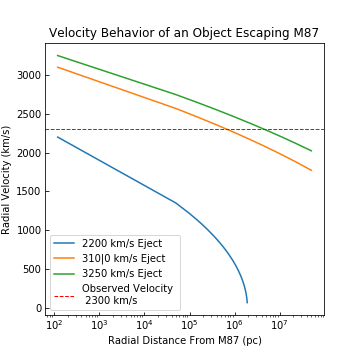
\includegraphics[width=6.4cm, height=6.4cm]{./Images/velocity_behavior.png}
    \centering
  \end{columns}
\end{frame}

\begin{frame}
  {Two Simulated Encounters of Interest}
  \begin{itemize}
    \item Ejected: 3400 km/s, Tidal Perturbation: about 100,000 times internal acceleration
    \item Ejected: 2400 km/s, Tidal Perturbation: about 13,000 times internal acceleration
  \end{itemize}

\end{frame}

\backupbegin

\begin{frame}
  {}
  \begin{center}
    \Huge Backup Slides
  \end{center}
\end{frame}

\subsection{}
\begin{frame}
  {3:1 Mass ratio}
  \begin{columns}
    \column{0.5\textwidth}
    \begin{itemize}
      \item 2-3 pc pass from larger BH.
      \item Tidal radius of 0.3-0.4 pc
    \end{itemize}
    \column{0.6\textwidth}
    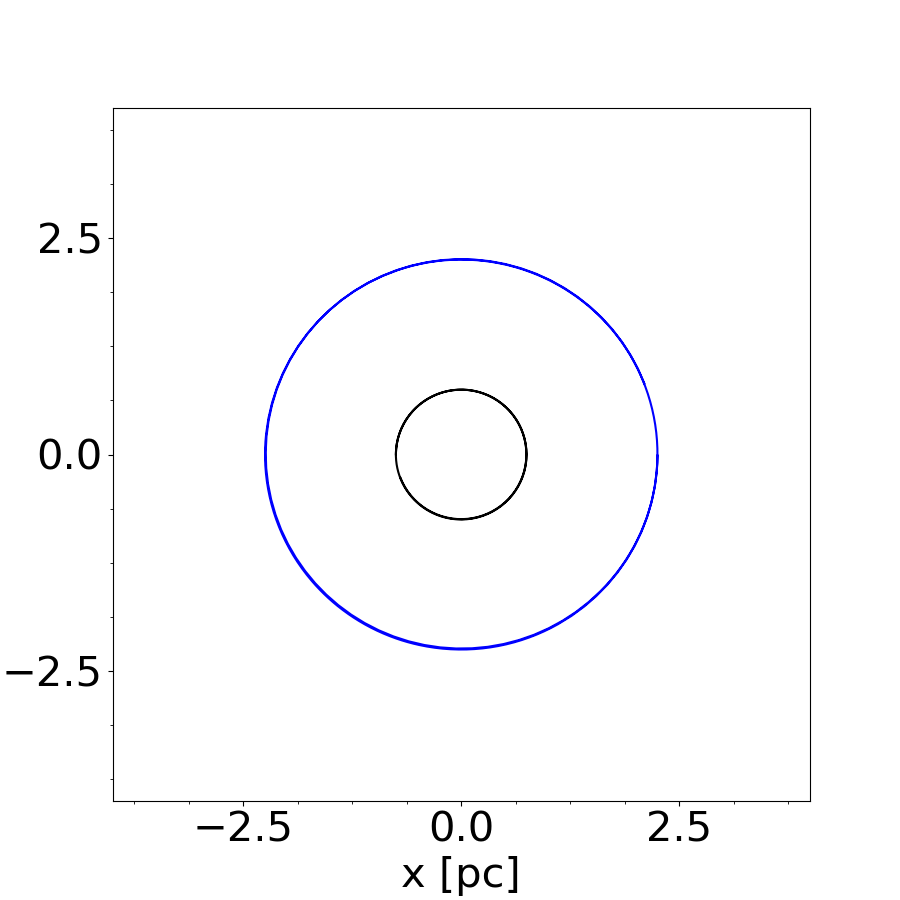
\includegraphics[width=6cm, height=6cm]{./Images/hvgc1_0333ratio.png}
    \centering
  \end{columns}
\end{frame}

\backupend
\end{document}